\subsubsection{Architecture of the Neural Language Model}\label{sec:architecture-of-the-neural-language-model}

After understanding the motivation behind Bengio et al. (2003), we can now study the architecture itself. The goal of the model is simple: \textbf{given the previous $n-1$ words, predict the next word}. For a training example:
\begin{equation*}
    \left(w_{t-N+1}, \dots, w_{t-1}, w_t\right)
\end{equation*}
The model receives the context:
\begin{equation*}
    \left(w_{t-N+1}, \dots, w_{t-1}\right)
\end{equation*}
And tries to predict the next word $w_t$. The complete architecture consists of four main components (see \autoref{fig:neural-language-model-architecture}):
\begin{enumerate}
    \item \important{Input Layer}. The input layer contains the \textbf{context words}. The dimension of the input layer is:
    \begin{equation*}
        \left|\text{Input Layer}\right| = \left(n-1\right) \cdot \left|V\right|
    \end{equation*}
    Where $n-1$ is the \textbf{number of context words} and $\left|V\right|$ is the \textbf{vocabulary size}.

    \highspace
    Here, nothing is stored. The input layer contains only identifiers, which are the indices of the context words in the vocabulary. The input layer is a \hl{one-hot representation} of the context words, where each word is represented as a vector of length $\left|V\right|$ with all zeros except for a single one at the index corresponding to the word in the vocabulary. As we saw in One-Hot Encoding, this representation is very sparse and high-dimensional (i.e., it has many zero entries). Therefore, the \textbf{network does not use these vectors as meaningful features}. Instead, they are simply fed to the next layer, the \textbf{embedding layer}.
    
    
    \item \important{Embedding (Projection) Layer}. Where the magic happens. The model contains a \textbf{trainable matrix}:
    \begin{equation*}
        C \in \mathbb{R}^{\left|V\right| \times m}
    \end{equation*}
    Where $\left|V\right|$ is the vocabulary size and $m$ is the \textbf{embedding dimension}, which is a hyperparameter that we can choose (e.g., $m=100$) and is typically much smaller than $\left|V\right|$, $m \ll \left|V\right|$. This matrix is called the \definition{Embedding Matrix} and each row corresponds to one word.
    
    \highspace
    \textcolor{Green3}{\faIcon{tachometer-alt} \textbf{Lookup Operation.}} Suppose the word \emph{Obama} corresponds to row $537$ in the embedding matrix $C$. Its one-hot vector will have a one at index $537$ and zeros everywhere else:
    \begin{gather*}
        \text{One-Hot}(\emph{Obama}) = [0^{(0)}, \dots, 1^{(537)}, \dots, 0^{(\left|V\right|-1)}] \\
        C = \begin{bmatrix}
            \vdots \\
            C_{537} \\
            \vdots
        \end{bmatrix} \xrightarrow{\text{lookup}} C(\emph{Obama}) = C_{537} \in \mathbb{R}^m
    \end{gather*}
    And the \hl{same applies to all other words in the context}. The embedding layer performs a \textbf{lookup} in the embedding matrix $C$ for each context word, retrieving their corresponding embedding vectors. Due to the lookup operation, this layer is called \textbf{projection}, since it projects the high-dimensional one-hot vectors into a lower-dimensional embedding space $\mathbb{R}^{\left|V\right|} \to \mathbb{R}^m$.

    \highspace
    \textcolor{Green3}{\faIcon{link} \textbf{Concatenation.}} After retrieving the embeddings, the model concatenates them. Suppose we have a context of $n-1=3$ words, the concatenation operation is:
    \begin{gather*}
        C\left(w_{t-3}\right) = \begin{bmatrix}
            0.1 \\
            0.5
        \end{bmatrix}
        \quad
        C\left(w_{t-2}\right) = \begin{bmatrix}
            0.3 \\
            0.7
        \end{bmatrix}
        \quad
        C\left(w_{t-1}\right) = \begin{bmatrix}
            0.2 \\
            0.4
        \end{bmatrix} \\
        x = \begin{bmatrix}
            C\left(w_{t-3}\right) \\
            C\left(w_{t-2}\right) \\
            C\left(w_{t-1}\right)
        \end{bmatrix} = \begin{bmatrix}
            0.1 \\
            0.5 \\
            0.3 \\
            0.7 \\
            0.2 \\
            0.4
        \end{bmatrix} \in \mathbb{R}^{(n-1) \cdot m}
    \end{gather*}
    The \textbf{concatenation} is important because it \hl{preserves the order of the context words}, which is crucial for language modeling. The resulting vector $x$ is then fed to the next layer, the \textbf{hidden layer}. Its dimension is:
    \begin{equation*}
        \left|\text{Embedding Layer}\right| = \left(n-1\right) \cdot m
    \end{equation*}
    Where $n-1$ is the number of context words and $m$ is the embedding dimension for each word.
    
    
    \item \important{Hidden Layer}. The purpose of the hidden layer is the classical one: \textbf{learns interactions between context words}. The hidden layer is a \textbf{fully connected layer} with a \textbf{nonlinear activation function}, typically $\tanh$ (\autopageref{sec:tanh-activation-function}). The hidden layer computes:
    \begin{equation*}
        h = \tanh\left(d + Hx\right)
    \end{equation*}
    Where $H \in \mathbb{R}^{h \times (n-1) \cdot m}$ is the \textbf{projection-to-hidden weight matrix}, $d \in \mathbb{R}^h$ is the \textbf{bias vector}, and $h$ is the number of \textbf{hidden units}, which is a hyperparameter that we can choose ($500 < h < 1000$). The hidden layer captures complex relationships between the context words and transforms the concatenated embeddings into a higher-level representation that is more suitable for predicting the next word. Its dimension is:
    \begin{equation*}
        \left|\text{Hidden Layer}\right| = h
    \end{equation*}

    
    \item \important{Output Layer}. The \textbf{final layer predicts the next word}. Its output size equals the vocabulary size $\left|V\right|$. For example, if the vocabulary size is $10,000$, then the network produces a vector of $10,000$ scores, one for each word in the vocabulary.
    
    \highspace
    These scores are converted into probabilities using the \textbf{softmax function} (\autopageref{def:softmax-activation-function}):
    \begin{equation*}
        \hat{P}\left(w_i = w_t \mid w_{t-N+1}, \ldots, w_{t-1}\right) = \frac{\exp\left(y_i\right)}{\sum_{j=1}^{\left|V\right|} \exp\left(y_j\right)}
    \end{equation*}
    \textcolor{Green3}{\faIcon{question-circle} \textbf{Why Softmax?}} Because softmax guarantees:
    \begin{equation*}
        0 \leq P\left(w_i\right) \leq 1 \quad \text{and} \quad \sum_i P\left(w_i\right) = 1
    \end{equation*}
    The output therefore becomes a proper probability distribution.
\end{enumerate}

\begin{figure}[!htp]
    \centering
    \resizebox{\textwidth}{!}{
        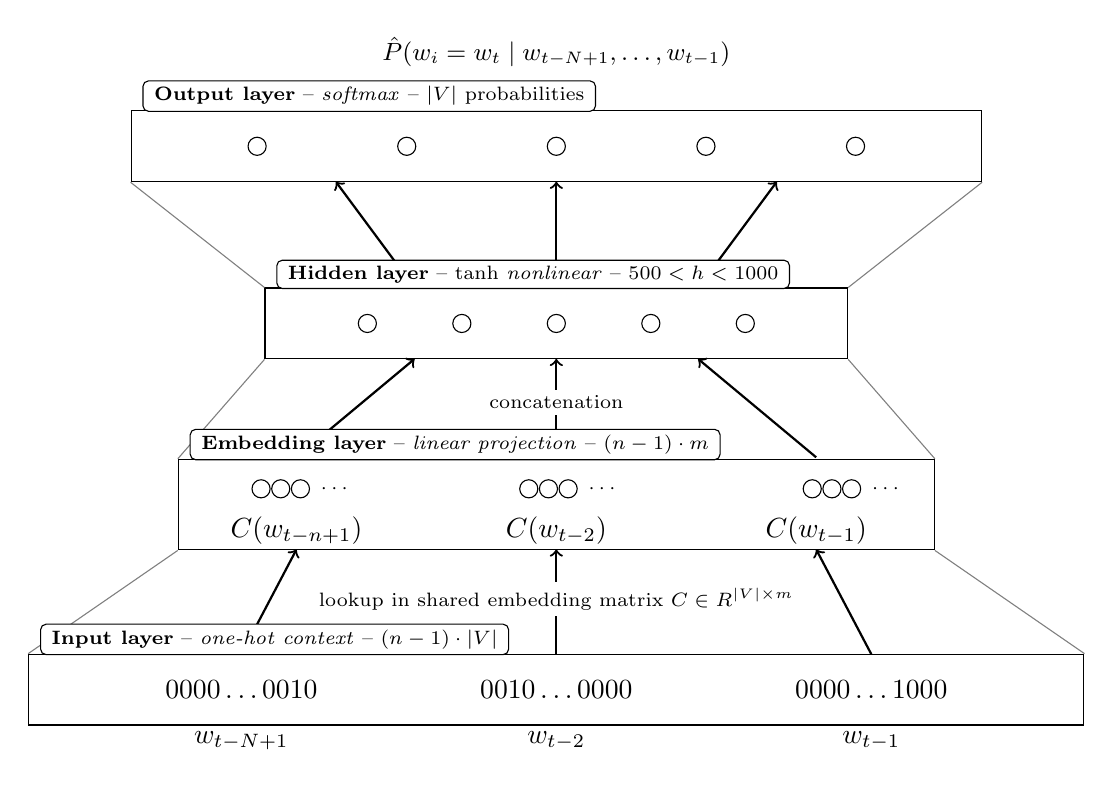
\begin{tikzpicture}[
            layer/.style={
                draw,
                minimum height=0.95cm,
                align=center
            },
            neuron/.style={
                circle,
                draw,
                minimum size=0.23cm,
                inner sep=0pt
            },
            arrow/.style={
                ->,
                thick
            },
            tag/.style={
                draw,
                rounded corners=2pt,
                fill=white,
                font=\scriptsize,
                inner xsep=4pt,
                inner ysep=2pt
            },
            smalltext/.style={
                font=\scriptsize,
                fill=white,
                inner sep=2.2pt
            }
        ]

            % -------------------------------------------------
            % Layer boxes
            % -------------------------------------------------

            \node[layer, minimum width=13.4cm, minimum height=0.9cm]  (input)     at (0,0) {};
            \node[layer, minimum width=9.6cm,  minimum height=1.15cm] (embedding) at (0,2.35) {};
            \node[layer, minimum width=7.4cm,  minimum height=0.9cm]  (hidden)    at (0,4.65) {};
            \node[layer, minimum width=10.8cm, minimum height=0.9cm]  (output)    at (0,6.9) {};

            % -------------------------------------------------
            % Input layer content
            % -------------------------------------------------

            \node at (-4.0,0) {$0000\ldots0010$};
            \node at (0,0)    {$0010\ldots0000$};
            \node at (4.0,0)  {$0000\ldots1000$};

            \node at (-4.0,-0.65) {$w_{t-N+1}$};
            \node at (0,-0.65)    {$w_{t-2}$};
            \node at (4.0,-0.65)  {$w_{t-1}$};

            % -------------------------------------------------
            % Lookup arrows and shared matrix label
            % -------------------------------------------------

            \draw[arrow] (-4.0,0.45) -- (-3.3,1.78);
            \draw[arrow] (0,0.45)    -- (0,1.78);
            \draw[arrow] (4.0,0.45)  -- (3.3,1.78);

            \node[smalltext] at (0,1.15) {
                lookup in shared embedding matrix $C \in \mathbb{R}^{|V|\times m}$
            };

            % -------------------------------------------------
            % Embedding layer content
            % -------------------------------------------------

            % Left embedding vector
            \foreach \x in {-3.75,-3.50,-3.25}
                \node[neuron] at (\x,2.55) {};
            \node[font=\scriptsize] at (-2.82,2.55) {$\cdots$};

            % Middle embedding vector
            \foreach \x in {-0.35,-0.10,0.15}
                \node[neuron] at (\x,2.55) {};
            \node[font=\scriptsize] at (0.58,2.55) {$\cdots$};

            % Right embedding vector
            \foreach \x in {3.25,3.50,3.75}
                \node[neuron] at (\x,2.55) {};
            \node[font=\scriptsize] at (4.18,2.55) {$\cdots$};

            % Embedding labels
            \node at (-3.3,2.02) {$C(w_{t-n+1})$};
            \node at (0,2.02)    {$C(w_{t-2})$};
            \node at (3.3,2.02)  {$C(w_{t-1})$};

            % -------------------------------------------------
            % Concatenation
            % -------------------------------------------------

            % Draw arrows first
            \draw[arrow] (-3.3,2.95) -- (-1.8,4.2);
            \draw[arrow] (0,2.95)    -- (0,4.2);
            \draw[arrow] (3.3,2.95)  -- (1.8,4.2);

            % Draw label after arrows to cut the central arrow
            \node[smalltext] at (0,3.65) {concatenation};

            % -------------------------------------------------
            % Hidden layer
            % -------------------------------------------------

            \foreach \x in {-2.4,-1.2,0,1.2,2.4}
                \node[neuron] at (\x,4.65) {};

            % -------------------------------------------------
            % Hidden to output
            % -------------------------------------------------

            \draw[arrow] (-1.8,5.1) -- (-2.8,6.45);
            \draw[arrow] (0,5.1)    -- (0,6.45);
            \draw[arrow] (1.8,5.1)  -- (2.8,6.45);

            % -------------------------------------------------
            % Output layer
            % -------------------------------------------------

            \foreach \x in {-3.8,-1.9,0,1.9,3.8}
                \node[neuron] at (\x,6.9) {};

            \node[font=\small] at (0,8.10) {
                $\hat{P}(w_i = w_t \mid w_{t-N+1},\ldots,w_{t-1})$
            };

            % -------------------------------------------------
            % Compression / expansion shape
            % -------------------------------------------------

            \draw[thin, gray] (input.north west) -- (embedding.south west);
            \draw[thin, gray] (input.north east) -- (embedding.south east);

            \draw[thin, gray] (embedding.north west) -- (hidden.south west);
            \draw[thin, gray] (embedding.north east) -- (hidden.south east);

            \draw[thin, gray] (hidden.north west) -- (output.south west);
            \draw[thin, gray] (hidden.north east) -- (output.south east);

            % -------------------------------------------------
            % Layer tags drawn last
            % -------------------------------------------------

            \node[tag, anchor=south west] at ([xshift=0.15cm,yshift=-0.02cm] input.north west)
                {\textbf{Input layer} -- \emph{one-hot context} -- $(n-1)\cdot |V|$};

            \node[tag, anchor=south west] at ([xshift=0.15cm,yshift=-0.02cm] embedding.north west)
                {\textbf{Embedding layer} -- \emph{linear projection} -- $(n-1)\cdot m$};

            \node[tag, anchor=south west] at ([xshift=0.15cm,yshift=-0.02cm] hidden.north west)
                {\textbf{Hidden layer} -- $\tanh$ \emph{nonlinear} -- $500 < h < 1000$};

            \node[tag, anchor=south west] at ([xshift=0.15cm,yshift=-0.02cm] output.north west)
                {\textbf{Output layer} -- \emph{softmax} -- $|V|$ probabilities};
        \end{tikzpicture}
    }
    \caption{Neural probabilistic language model architecture inspired by Bengio et al. (2003).}
    \label{fig:neural-language-model-architecture}
\end{figure}

\begin{flushleft}
    \textcolor{Green3}{\faIcon{question-circle} \textbf{How do we measure whether the prediction is good?}}
\end{flushleft}
Suppose the model predicts:
\begin{center}
    \begin{tabular}{@{} l l @{}}
        \toprule
        \textbf{Word} & \textbf{Predicted Probability} \\
        \midrule
        \emph{sleeps} & $0.8$ \\
        \bottomrule
    \end{tabular}
\end{center}
\noindent
This is very good. Instead, suppose the model predicts:
\begin{center}
    \begin{tabular}{@{} l l @{}}
        \toprule
        \textbf{Word} & \textbf{Predicted Probability} \\
        \midrule
        \emph{sleeps} & $0.01$ \\
        \bottomrule
    \end{tabular}
\end{center}

\newpage

\noindent
This is terrible. We therefore need a loss function that:
\begin{itemize}
    \item Is \textbf{small} when the correct word has \textbf{high probability};
    \item Is \textbf{large} when the correct word has \textbf{low probability}.
\end{itemize}
The Bengio's paper uses the \textbf{negative log-likelihood loss}:
\begin{equation}
    E = -\log \hat{P}\left(w_t \, | \, w_{t-N+1}, \dots, w_{t-1}\right)
\end{equation}
This loss function has the desired properties:
\begin{itemize}
    \item \textbf{Very good prediction}:
    \begin{equation*}
        P\left(w_t \, | \, \text{context}\right) = 0.9
    \end{equation*}
    Then the loss is:
    \begin{equation*}
        E = -\log\left(0.9\right) \approx 0.105
    \end{equation*}
    Small error.
    \item \textbf{Mediocre prediction}:
    \begin{equation*}
        P\left(w_t \, | \, \text{context}\right) = 0.5
    \end{equation*}
    Then the loss is:
    \begin{equation*}
        E = -\log\left(0.5\right) \approx 0.693
    \end{equation*}
    Larger error.
    \item \textbf{Terrible prediction}:
    \begin{equation*}
        P\left(w_t \, | \, \text{context}\right) = 0.01
    \end{equation*}
    Then the loss is:
    \begin{equation*}
        E = -\log\left(0.01\right) \approx 4.605
    \end{equation*}
    Huge error.
\end{itemize}
In other words, Bengio's idea was to \hl{punish the network when it assigns a low probability to the correct next word}.